
\documentclass[fleqn]{exam}
\usepackage{amsmath}
\usepackage{graphicx}
\usepackage{booktabs}
\usepackage{float}
\usepackage{caption}
\usepackage{polynom}
\usepackage{mdwlist}
\usepackage{cancel}
\usepackage{fullpage}

\usepackage{parskip}
\usepackage{paralist}

\usepackage{unitsdef} 
\newunit{\inch}{in}
\newunit{\mile}{mile}
\newunit{\mph}{mph}
\newunit{\foot}{ft}
\newunit{\knot}{knot}
\newunit{\gallon}{gallon}

\setcounter{tocdepth}{2}

\everymath{\displaystyle}


% \begin{figure}[H]
%   \centering
%   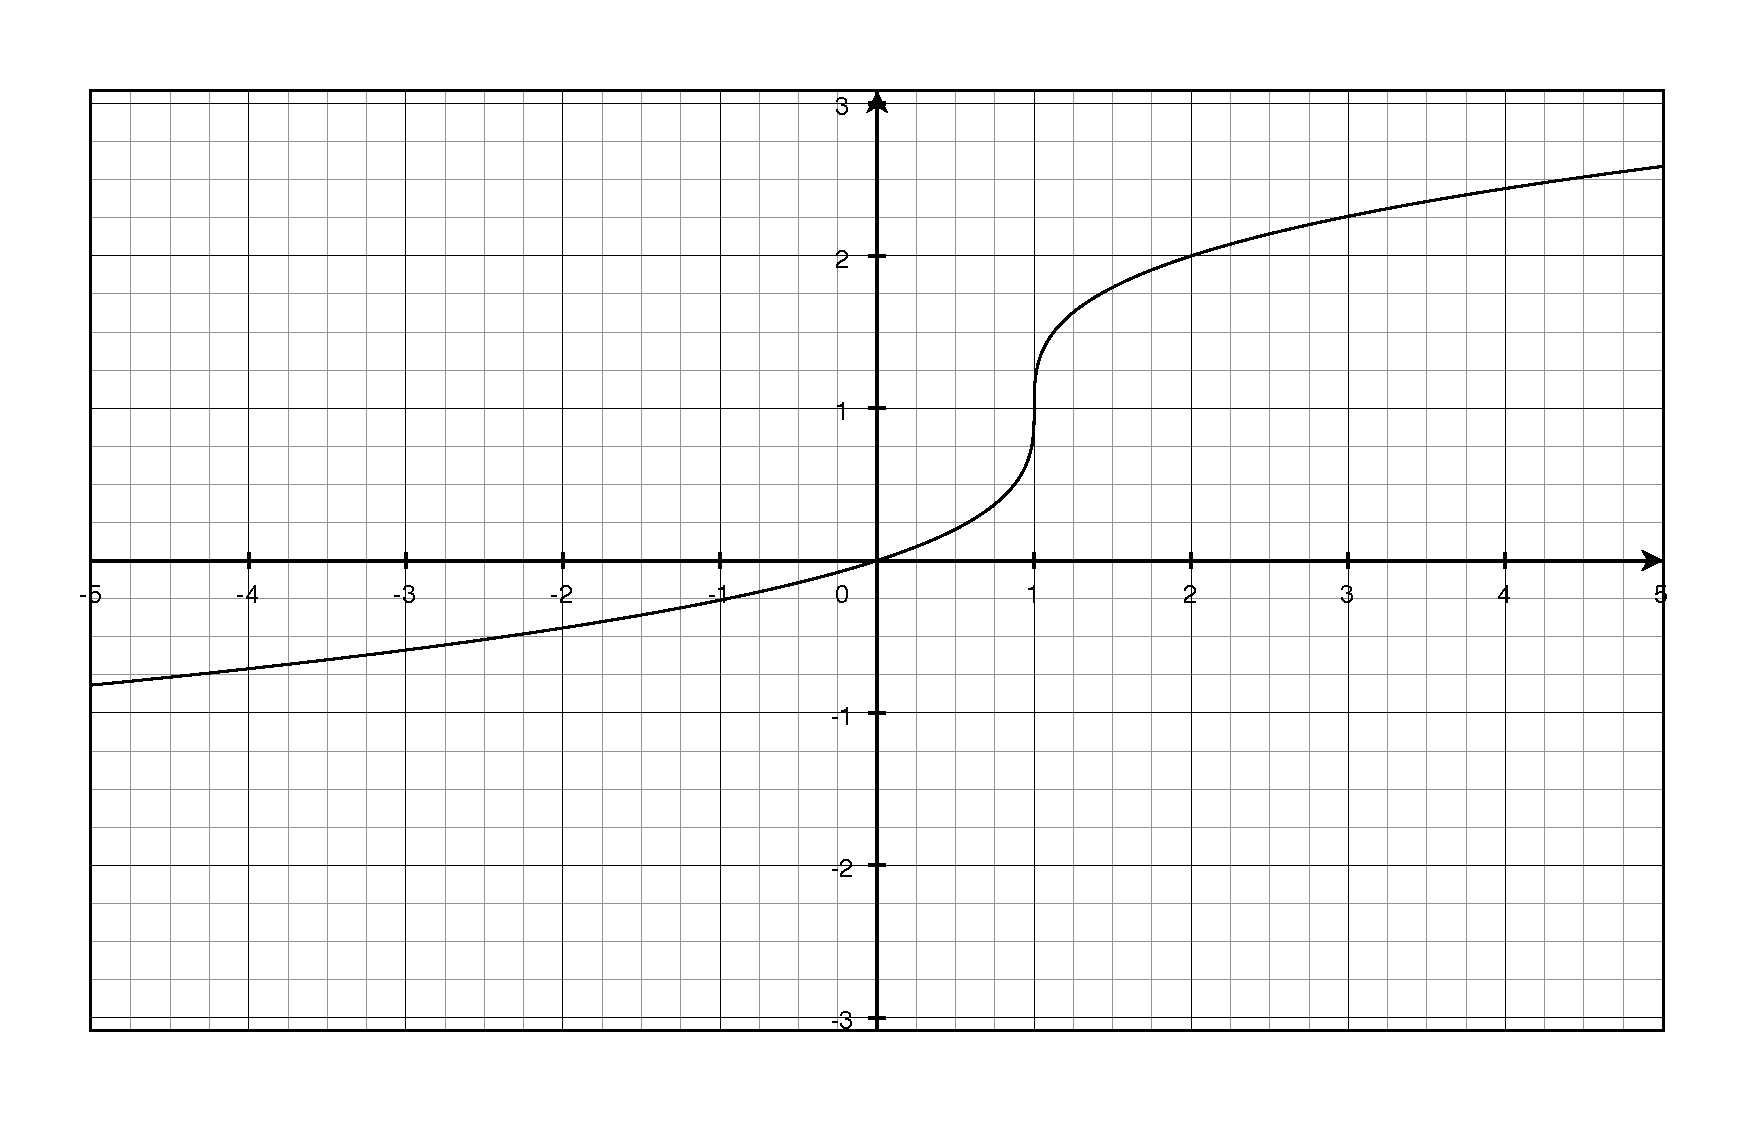
\includegraphics[scale=.3]{question7.eps}
%   \caption*{Question 7}
% \end{figure}

% \begin{tabular}{cc}
% \toprule
% period & amplitude \\
% \midrule
%   $\pi$ & $2$ \\
% \bottomrule
% \end{tabular}

\printanswers

%% \ifprintanswers
%% \usepackage{2in1, lscape}
%% \fi

\title{Math 263A \\ Chapter Two Study Guide \\ Limits and Continuity}
\date{September 29, 2012}

\author{}

\begin{document}

\maketitle  

% \tableofcontents

\section{Limits}

The informal definition of
\[
  \lim_{x \to a} f(x) = c
\]
is that as $x$ gets closer to $a$, $f(x)$ gets closer to $c$.  You can make $f(x)$ as close to $c$ as you want by
selecting a value of $x$ close enough to $a$.

The value of $f$ at $a$ doesn't matter at all, and $f$ doesn't even have to be defined at $a$.  Only values close to $a$
matter.

Sometimes the value that $f(x)$ approaches as you go up to $a$ from the left is different from the value that $f(x)$
approaches as you descend to $a$ from the right.  If this happens, $\lim_{x \to a} f(x)$ isn't defined, but 
$\lim_{x \to a-} f(x)$ (from the left) and/or $\lim_{x \to a+} f(x)$ (from the right) may be defined.

Sometimes the function doesn't settle in on a particular value, so the limit isn't defined.  An example of this is 
$f(x) = \sin \left( \frac{1}{x} \right)$.  See the graph on page 68.

Limits behave just like you would expect.  The rules are all given on page 79, but they mostly follow common sense.  For
example, if you multiply a function by a constant value, the new limit is the original limit multipled by the same
constant value.

To find the limit of a polynomial function, just plug the limit value in the function.  For example:
\[
  \lim_{x \to 2} x^2 + 2x + 1 = 9
\]

If you have a rational function and plugging the limit value in would make both the numerator and denominator zero, try
\begin{itemize*}
  \item factor the numerator and denominator
  \item cancel factors that appear in both the numerator and denominator
  \item see if the denominator is no longer zero when you plug in the limit value. 
\end{itemize*}

For example:
\begin{align*}
  \lim_{x \to 2} \frac{x^2 - 4}{x - 2} = \lim_{x \to 2} \frac{(x + 2)(x - 2)}{x - 2} = \lim_{x \to 2} x + 2 = 4
\end{align*}

\section{Continuity}

A function is continuous if, naturally enough, the graph of the function doesn't contain any gaps.  This happens when
the value of the function at every point is equal to the limit as you approach the point.  Or, as an equation:
\[
  \lim_{x \to c} f(x) = f(c)
\]
for every $c$ in the interval in which you are interested.  Of course, this means that the function must also be defined
for every value in the interval in which you are interested.

If you have an open interval, the endpoints don't matter.  For a closed interval, $[a, b]$, the function must be right
continuous at $a$ and left continuous at $b$.

If a $f$ and $g$ are both continuous at $c$, then: $f + g$, $f - g$, $fg$, $f/g$, $kf$, $f^n$ are all also continuous at
$c$, provided, of course, that they are still defined at $c$.

If $f$ is continous at $c$ and $g(f(c))$ is continuous at $f(c)$, then $g \circ f$ is continuous at $c$.  This is
useful for things like:
\[
  h(x) = | \sin x + \cos x |
\]
You can think of this as $f(x) = \sin x + \cos x$ and $g(x) = |x|$.  Since both functions are continuous everywhere, the
composition of the two functions is also continuous everywhere.

%% \subsection{Examples}

%% \begin{enumerate}
%% \item
%% Is this function continuous at 2?
%% \[
%%   f(x) = \frac{x^2 - 4}{x - 2}
%% \]
%% \begin{solution}
%%   No, because the function is not defined at $x = 2$.
%% \end{solution}

%% \item
%% How would you define $f(2)$ to make make $f$ continuous at 2?
%% \[
%%   f(x) = \frac{x^2 - 4}{x - 2}
%% \]
%% \begin{solution}
%% \[
%%   \lim_{x \to 2} \frac{x^2 - 4}{x - 2} =   \lim_{x \to 2} x + 2 = 4
%% \]
%% So if $f(2)$ is defined to be 4, the function becomes continuous at 2.
%% \end{solution}

%% \end{enumerate}

\section{Intermediate Value Theorem}
The {\em Intermediate Value Theorem} says that if $f$ is continuous on $[a, b]$ then for any number $W$ between $f(a)$ and
$f(b)$ there is some $c$ such that $f(c) = W$.  

This is just common sense expressed as a theorem.  All it is really saying is that if, for example, are stationary at
time 0 and are moving at 60 mph 10 seconds later, some time during those 10 seconds you were traveling at 30 mph, or 28
mph, or whatever speed between 0 and 60 mph you can think of.  This only works for continuous functions like car
speeds.  If you have access to Star Trek's warp drive, you may not hit all the speeds between 0 and warp 5, although I'm
not entirely clear on how the warp drive operates.

\end{document}
